\begin{figure}[htbp]
\centering
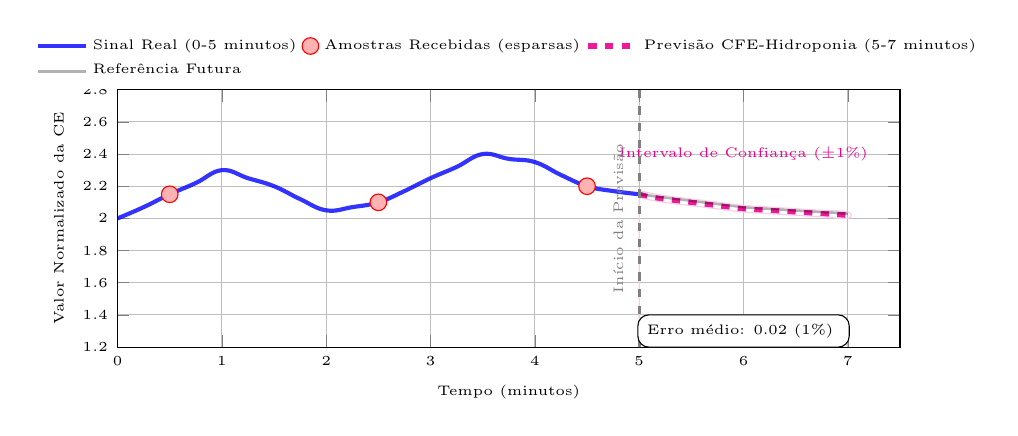
\begin{tikzpicture}
\begin{axis}[
    width=0.95\textwidth,
    height=0.40\textwidth,
    xlabel={Tempo (minutos)},
    ylabel={Valor Normalizado da CE},
    grid=major,
    legend style={at={(0.5,-0.15)}, anchor=north, legend columns=2},
    xmin=0, xmax=7.5,
    ymin=1.2, ymax=2.8,
    xtick={0,1,2,3,4,5,6,7},
    ytick={1.2,1.4,1.6,1.8,2.0,2.2,2.4,2.6,2.8},
    tick label style={font=\tiny},
    label style={font=\tiny},
    legend style={font=\tiny},
    legend cell align=left,
    legend style={
        at={(0.5,1.)},
        anchor=south,
        legend columns=3,
        font=\tiny,
        draw=none
    },
    % title={Capacidade Preditiva para Períodos Futuros Não Medidos},
    % title style={font=\large\bfseries, yshift=8pt}
]

% Sinal Real (0-5 minutos) - Mais pontos para suavização melhor
\addplot[smooth, tension=0.7, blue, line width=1.5pt, opacity=0.8] coordinates {
    (0.00, 2.00) (0.25, 2.07) (0.50, 2.15) (0.75, 2.22) (1.00, 2.30)
    (1.25, 2.25) (1.50, 2.20) (1.75, 2.12) (2.00, 2.05) (2.25, 2.07)
    (2.50, 2.10) (2.75, 2.17) (3.00, 2.25) (3.25, 2.32) (3.50, 2.40)
    (3.75, 2.37) (4.00, 2.35) (4.25, 2.27) (4.50, 2.20) (4.75, 2.17)
    (5.00, 2.15)
};
\addlegendentry{Sinal Real (0-5 minutos)}

% Amostras Recebidas (esparsas)
\addplot[only marks, mark=*, mark size=3pt, color=red, fill=red!30] coordinates {
    (0.5, 2.15) (2.5, 2.10) (4.5, 2.20)
};
\addlegendentry{Amostras Recebidas (esparsas)}

% Previsão CFE-Hidroponia (5-7 minutos) - Mais pontos
\addplot[smooth, tension=0.8, magenta, dashed, line width=2pt, opacity=0.9] coordinates {
    (5.00, 2.15) (5.12, 2.13) (5.25, 2.12) (5.38, 2.11) (5.50, 2.10)
    (5.62, 2.09) (5.75, 2.08) (5.88, 2.07) (6.00, 2.06) (6.12, 2.055)
    (6.25, 2.05) (6.38, 2.045) (6.50, 2.04) (6.62, 2.035) (6.75, 2.03)
    (6.88, 2.025) (7.00, 2.02)
};
\addlegendentry{Previsão CFE-Hidroponia (5-7 minutos)}

% Referência Futura - Mais pontos
\addplot[smooth, tension=0.8, black, line width=1pt, opacity=0.3] coordinates {
    (5.00, 2.15) (5.12, 2.14) (5.25, 2.13) (5.38, 2.12) (5.50, 2.11)
    (5.62, 2.10) (5.75, 2.09) (5.88, 2.08) (6.00, 2.07) (6.12, 2.065)
    (6.25, 2.06) (6.38, 2.055) (6.50, 2.05) (6.62, 2.045) (6.75, 2.04)
    (6.88, 2.035) (7.00, 2.03)
};
\addlegendentry{Referência Futura}

% Intervalo de Confiança com mais pontos para suavização
\addplot[smooth, tension=0.7, magenta!20, fill opacity=0.3] coordinates {
    (5.00, 2.1715) (5.25, 2.1412) (5.50, 2.1210) (5.75, 2.1008) (6.00, 2.0806)
    (6.25, 2.0705) (6.50, 2.0604) (6.75, 2.0503) (7.00, 2.0402)
    (7.00, 1.9998) (6.75, 2.0097) (6.50, 2.0196) (6.25, 2.0295) (6.00, 2.0394)
    (5.75, 2.0592) (5.50, 2.0790) (5.25, 2.0988) (5.00, 2.1285)
} \closedcycle;

\node[font=\tiny, color=magenta] at (axis cs:6.0,2.4) {Intervalo de Confiança ($\pm$1\%)};

% Linha divisória entre passado e futuro
\draw[dashed, gray, line width=1.2pt] (5,1.2) -- (5,2.8);
\node[font=\tiny, color=gray, rotate=90] at (axis cs:4.8,2.0) {Início da Previsão};

% Anotação sobre precisão
\node[draw, fill=white, rounded corners, font=\tiny, align=center] at (axis cs:6.0,1.3) {
    Erro médio: 0.02 (1\%)
};

\end{axis}
\end{tikzpicture}
\caption{Capacidade preditiva do sinal transmitido via CFE-HYDRO para horizontes futuros curtos (2 minutos). O sistema demonstra maior precisão mesmo com amostragem esparsa, mantendo erro abaixo de 1\%.}
\label{fig:capacidade_preditiva}
\end{figure}
